 \documentclass{article} % For LaTeX2e
\usepackage{cos424,times}
\usepackage{hyperref}
\usepackage{url}
\usepackage{graphicx}
\usepackage{amsmath}
\usepackage{multirow}
\usepackage{parskip}
\usepackage{placeins}

\bibliographystyle{plos2009}


\title{Clustering Last.fm Users}


\author{
Ava Chen\\
Department of Computer Science\\
\texttt{avac@princeton.edu}\\
\And
James Bartusek\\
Department of Computer Science\\
\texttt{bartusek@princeton.edu} \\
\And
Nabeel Sarwar\\
Department of Astrophysical Sciences\\
\texttt{nsarwar@princeton.edu} \\
}

\newcommand{\fix}{\marginpar{FIX}}
\newcommand{\new}{\marginpar{NEW}}

\begin{document}

\maketitle

\begin{abstract}
\end{abstract}


\section{Introduction}

Last.fm (\cite{lastfm}) is a music website that collects music preference information for its users. Users will have preferrered artists, how many times they listen to them, and what events they attend. Using this information, Last.fm generates music recommendations for each user. Last.fm is also tied in with different people's social media networks, so for each user, a large number of features are collected. For each user, we can collect the number of times that they listen to each artist. In this project, we use data collected from the Fall of 2008 and cleaned in 2009 to analyze how users cluster into various artists.  

This data is naturally sparse as most users do not listen to many artists. There are, however, many 

\section{Data processing}

We limited the number of artists based on the number of unique users that listened to an artist. The 1000 artists with the highest number of unique users are used as the features for each user. The goal of this was to remove artists that are popular among only among very few number of users. 

The data is from \cite{data}. The number of users is that have listened to these artists are 9809. 


\section{Clustering Methods}


We cluster the data using two EM algorithms and using a soft EM K-means algorithm. To cluster the users, the number of times each users has listened to each artist is used as the features. 


\begin{itemize}
    \item K-means with 20 components
    \item Gaussian Mixture Model with 10 components
    \item Poisson Mixture 10 components
\end{itemize}

K-means was used a naive model that could be compared to the Gaussian Mixture and Poisson Mixture models. For each clustering method, we calculate the silhouette score. 

Both the K-means algorithm and the Gaussian Mixture Model for clustering were implemented in \cite{scikit-learn}. 

The Poisson Mixture is used as the data is count data. It is not unreasonble that the counts that an artist is listened to by a user is Poisson distributed. The Poisson mixture model used calculated cluster groups using an EM algorithm. So with this assumption, listening to an artist is viewed as a Poisson process. 

\section{Imputation Methods}
To imputate the 

\begin{itemize}
    \item K-means imputation
    \item GMM Imputation
    \item Singular Value Decomposition
    \item Non-negative matrix factorization using nonnegative double singular value decompositions
\end{itemize}
\section{Results}



\subsection{Clusters}
For

\subsection{Imputation}
Using matrix various matrix factorization methods, we imputated the interaction rate between a user and an artist. Here we will report the violin plots and the area under curve for the precision-recall curve. 

\begin{itemize}
    \item 
\end{itemize}

\begin{figure}
\centering
\includegraphics[width=0.5\textwidth]{NMFdecompositionROC.png}
\caption{\textbf{Violin Plots of .}  }
\label{fig:ROCNMF}
\end{figure}

\begin{figure}
    \centering
    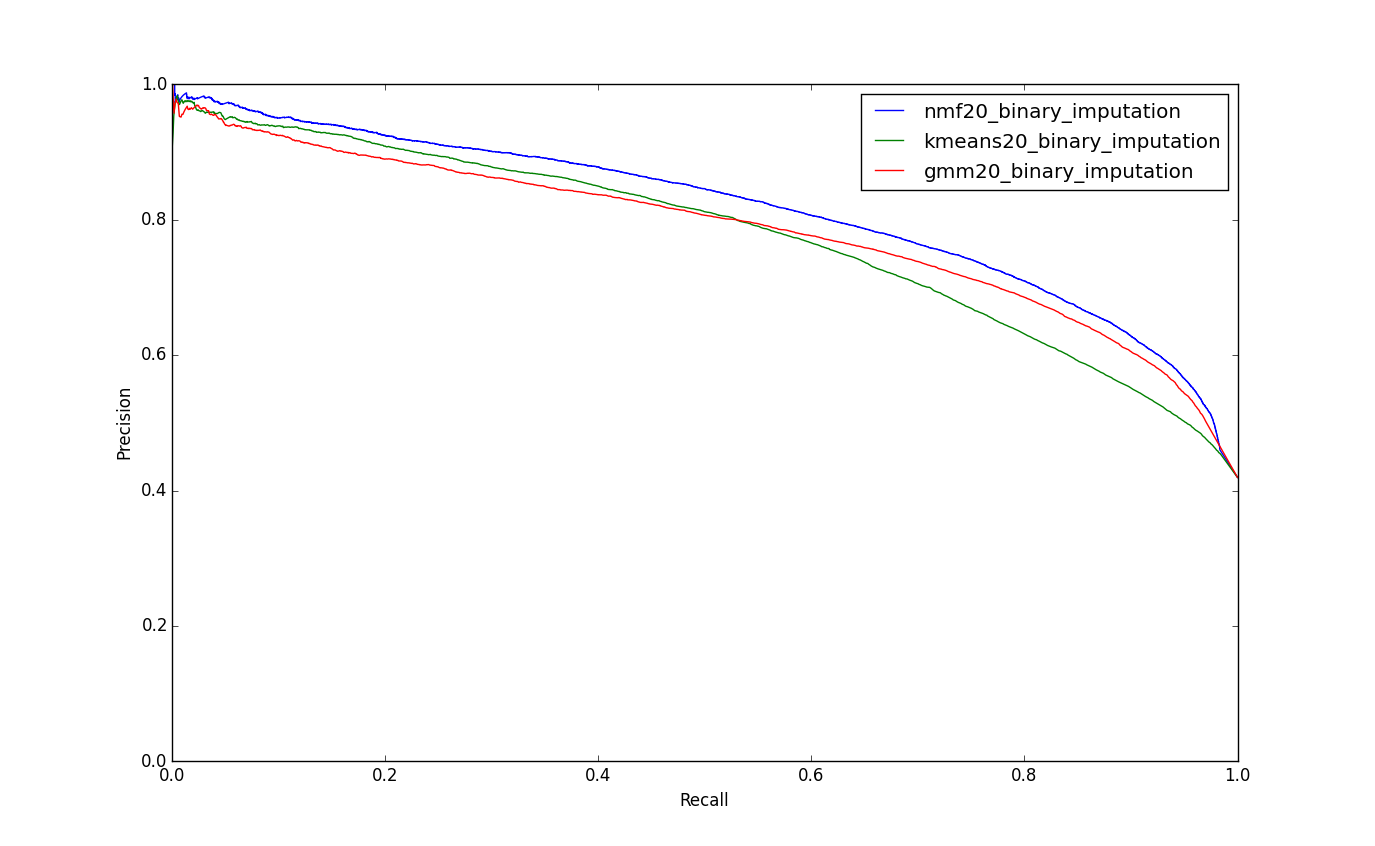
\includegraphics[width=0.5\textwidth]{methods_pr-binary-imputation.png}
    \caption{\textbf{Precision and Recall} for the different imputation methods. NMF had the best peformance}
    \label{fig:precisionrecall}
\end{figure}

\begin{table}[htbp]
\small
   \centering
   \begin{tabular}{@{}|c|c|c|@{}} % Column formatting, @{} suppresses leading/trailing space 
   \hline
  Method & & Prec & Recall & $F_1$ & r-value  \\ \hline \hline
  SVD Imputation & 0.8996 & 0.4954 & 0.22 & 0.3047 & 0.2835 \\
  NMF Imputation & 0.9045 & 0.5413 & 0.2950 & 0.3819 & 0.3532\\
  NMF Imputation (sparse) & 0.9050 & 0.5462 & 0.2950 & 0.3819 & 0.3554 \\
  LDA Imputation (20 topics) & 0.845 & 0.223 & 0.222 & 0.2226 & 0.13658 \\
  LDA Imputation (15 topics) & 0.8286 & 0.2139 & 0.267 & 0.2375 & 0.1434 \\ \hline
   \end{tabular}
   \caption{{\bf Results of 4 different methods of matrix factorization.} } 
   \label{tab:methods}
\end{table}

\section{Conclusion and Extensions}


\bibliography{ref}

\end{document}


